%\documentclass[wcp,gray]{jmlr} % test grayscale version
\documentclass[10pt]{jmlr}% former name JMLR W\&CP
%\documentclass[pmlr]{jmlr}% new name PMLR (Proceedings of Machine Learning)

 % The following packages will be automatically loaded:
 % amsmath, amssymb, natbib, graphicx, url, algorithm2e
 \usepackage{amsmath,amssymb,graphicx,url}

 %\usepackage{rotating}% for sideways figures and tables
\usepackage{longtable}% for long tables

 % The booktabs package is used by this sample document
 % (it provides \toprule, \midrule and \bottomrule).
 % Remove the next line if you don't require it.
\usepackage{booktabs}
 % The siunitx package is used by this sample document
 % to align numbers in a column by their decimal point.
 % Remove the next line if you don't require it.
\usepackage[load-configurations=version-1]{siunitx} % newer version
 %\usepackage{siunitx}

% Package to make table with multi rows and columns
\usepackage{multirow}
 
 % to do
\usepackage{xcolor}
\newcommand\todo[1]{\textcolor{red}{#1}}

 % change the arguments, as appropriate, in the following:
\jmlrvolume{}
\jmlryear{}
\jmlrworkshop{STA723 -- Case Study 1}
\jmlrproceedings{}{}


\usepackage[toc,page]{appendix}



% start article
% \titlebreak
% \footnote{}
% \textsf

\title[DDE and PCB effect on Premature delivery]{Assessing Effects of Exposures to DDE and PCBs on Premature Delivery via Ordinal Logistic Regression}	%\titletag{\thanks{XXX}} % leave empty?

 % Use \Name{Author Name} to specify the name.
 % If the surname contains spaces, enclose the surname
 % in braces, e.g. \Name{John {Smith Jones}} similarly
 % if the name has a "von" part, e.g \Name{Jane {de Winter}}.
 % If the first letter in the forenames is a diacritic
 % enclose the diacritic in braces, e.g. \Name{{\'E}louise Smith}

 % Authors with different addresses:
 
 \author[Morsomme, Ou, Zito]{Raphael Morsomme \and Rihui Ou \and Alessandro Zito}
 \date{\today} % Date, can be changed to a custom date

 % Three or more authors with the same address:
 % \author{\Name{Author Name1} \Email{an1@sample.com}\\
 %  \Name{Author Name2} \Email{an2@sample.com}\\
 %  \Name{Author Name3} \Email{an3@sample.com}\\
 %  \addr Address}

 % Authors with different addresses:
 % \author{\Name{Author Name1} \Email{abc@sample.com}\\
 % \addr Address 1
 % \AND
 % \Name{Author Name2} \Email{xyz@sample.com}\\
 % \addr Address 2
 %}

% leave editor's section empty?
%\editor{Editor's name}
% \editors{List of editors' names}

\begin{document}

\maketitle

\begin{abstract}
This report focuses on the adverse effects of exposures to DDE and PCB chemicals on the chance of premature birth delivery, which may be associated to a weaker health status for the newborn. In particular, we analyze the gestation length in weeks of a sample 2380 women of different race and economic status collected across 11 medical centers. We first divide the women into three groups ("Dangerous preterm", "Preterm" and "At term").  As DDE and PCB are lipophilic substances, we correct their concentration measurement to control for an estimate of the lipids in the blood, and later use these adjusted measures as explanatory variables in a Bayesian ordinal logistic regression model with the women's group as outcome. We find that the effects of the chemicals are essentially race dependent: increases in PCB levels are more detrimental to non-whites, while increases in DDE enhance the odds of a more dangerous delivery on white. 
\end{abstract}
\newpage
%%%%%%%%%%%%%%%%%%%%%%%%%%%%%%%%%%%%%%%%%%%%%%%%%%%%%%%%%%%%%
% INTRODUCTION
%%%%%%%%%%%%%%%%%%%%%%%%%%%%%%%%%%%%%%%%%%%%%%%%%%%%%%%%%%%%%
\section{Introduction}
\label{sec:intro}

Dichlorodiphenyldichloroethylene (DDE) and Polychlorinated Biphenyls (PCB) are two chemical elements which were commonly useD in the United States for agricultural purpouses and were banned during the 70's due to their detrimental effect on human health. In particular, exposure to these chemical products has been linked to neurobehavioral and developmental deficits in newborns. As the human body stores them in its fatty tissues, studying their impact on human health is particularly important.

In this report, we examine the effect of DDE and PCB on fetuses; more precisely, we assess the potential association between the exposure to these chemicals and the chance of early delivery. Ideally, a higher exposure to the substances induces a preterm delivery, which may have adverse consequences for the child. To verify this theory, we construct an ordinal logistic regression model over three delivery groups defined by the recorded lenght of the gestation period.  We find that the impact of the substances is essentially race specific: exposure to DDE increases the risk of early childbirth among white people and exposure to PCB increases the risk among non-white ones. 

The report is divided as follows: \sectionref{sec:method} presents the data and our methodology,  \sectionref{sec:results} reports our findings, \sectionref{sec:conclusion} discusses the results and concludes.


%%%%%%%%%%%%%%%%%%%%%%%%%%%%%%%%%%%%%%%%%%%%%%%%%%%%%%%%%%%%%
% METHODS
%%%%%%%%%%%%%%%%%%%%%%%%%%%%%%%%%%%%%%%%%%%%%%%%%%%%%%%%%%%%%
\section{Methods}
\label{sec:method}

\subsection{Data}
\label{sec:data}
The data set consists of 2,380 pregnant women that visited a hospital during their pregnancy in 2001. It contains the length of the gestation in weeks, the concentration doses of DDE and the twelve PCB breakdown products in the blood, the concentration of cholesterol and triglycerides and several demographic information (race, level of education, income, occupation, age, smoking status and the center attended by the woman). However, 43 women showed a length of gestation superior to 45 weeks (the second longest gestation period ever recorded), and 1 women did not show any records of the PCBs levels. Thus, we decide to drop them, reducing the number of women to 2,336. Finally, we mean impute the missing data on the income, education and occupational scores\footnote{Note that these scores will not end up in the final model.}. The following subsection describes the construction of the relevant variable in our analysis.

\subsection{Feature Engineering}
\label{sec:feature}
As a first step, we divide the women into three groups, labelled as "Dangerous Preterm", "Preterm" and "At term" based upon the lenght of thei gestation (shorter than $33$ weeks, between $34$ and $36$ weeks and longer than $37$ weeks, respectively). The groups are mean to capture the danger associated to the birth for the child himself. While a delivery after 37 weeks is considered normal, the main organs (especially the respiratory system) develop between week 34 and 37, making a birth before 34 weeks more dangerous. Second, as the twelve PCB measurements showed a high correlation (see \figureref{fig:corr} in \appendixref{appendix:fig}), we aggregate them into a unique variable by taking their standardized average \footnote{We first standardize each single PCB to to prevent one measurement to dominate the aggregate variable.}. Third, we combine the measurements of chemical in blood with the fat-related variables to estimate the initial level of DDE and PCBs to which the women were exposed from the environment. In particular, we calculate the total amount of fatty tissues using the formula in \cite{Phillips1989} and \cite{Bernert2007}

\begin{equation}
\label{eq:fat}
\text{lipid} = 2.27 * \text{cholesterol} + \text{triglycerides} + 0.623.
\end{equation}
Then, since the amount of chemical absorbed is proportional to the amount of fatty tissue one has, we adjust the concentration of PCB and DDE in blood by dividing by the log of the level of lipid\footnote{This correction derives from a Box-Cox analysis of our model, following the basic procedure in \cite{Li_Long_Duns}. See the appendix for further details.}.
\begin{equation}
\label{eq:exp_dde_pcb}
\text{DDE}_{\text{exposure}} = \dfrac{\text{DDE}}{\log(\text{lipid})} \qquad \text{PCB}_{\text{exposure}} = \dfrac{\text{PCB}_\text{aggregate}}{\log(\text{lipid})}.
\end{equation}
Finally, we aggregate the women into two groups, "white" and "non-white", based on the reported race\footnote{The original data had 1,016 white women, 1,201 black ones, and 120 labelled as "other". As the categories are unbalanced, we prefer to merge for a clearer interpretation.}.

\subsection{Ordinal Logistic Regression Model}
$\text{DDE}_{\text{exposure}}$ and $\text{PCB}_{\text{exposure}}$ are our variables of interest, whereas the above constructed delivery group is our dependent variable. In order to identify non-spurious association between these variables and the occurrence of early deliveries, we run the following ordinal logistic regression model 

\begin{equation}
\label{eq:ordi_logit}
\text{logit}(P(gestgroup \le j)) = \beta_{0j} - \mathbf{X} \boldsymbol{\beta}
\end{equation}

for $j=0$ (=Dangerous)$,1$ (=Preterm), where $\beta_{j0}$ is the baseline coefficient for category $j$, $\boldsymbol{\beta}$ is the effect of each covariate on the log odds and $\mathbf{X}$ is the matrix of regressors. In order to incorporate the model uncertainty into the analysis, we adopt a Bayesian approach. In particular, we first run a forward and backward AIC-based variable selection, which leads to an $\mathbf{X}$ that includes $\text{DDE}_{\text{exposure}}$, $\text{PCB}_{\text{exposure}}$, smoke, center, race and the interactions between $(\text{DDE}_{\text{exposure}}$ and race and between $\text{PCB}_{\text{exposure}}$ and race.\footnote{Ideally, we wish to adopt a Bayesian model averaging (BMA) approach. However, as we are not aware of existing computing resources to apply BMA on an ordinal logistic regression model, we carry out the selection using a frequentist procedure. The variables dropped from the full model are three scores, mother age, and the interactions between $\text{DDE}_{\text{exposure}}$ and center, and between $\text{PCB}_{\text{exposure}}$ and center.}. Second, we set a uniform prior over each coefficent. To further check the robustness of the model, we apply a $R^2$-prior as well. The following section reports and summarises our findings. Ordinal logistic model assumptions are checked in the appendix.

%%%%%%%%%%%%%%%%%%%%%%%%%%%%%%%%%%%%%%%%%%%%%%%%%%%%%%%%%%%%%
% RESULTS
%%%%%%%%%%%%%%%%%%%%%%%%%%%%%%%%%%%%%%%%%%%%%%%%%%%%%%%%%%%%%
\section{Results}
\label{sec:results}

%%%%%%%%%%%%%%%%%%%%%%%%%%%%%%%%% EDA
\subsection{EDA}

\figureref{fig:corr} presents the correlation matrix of the $11$ PCB measurements. We can observe that they are highly correlated with each other. This is not surprising since they correspond to breakdown products of PCB. This provides a rationale for aggregating these measurements into one variable that attempts to approximate the total amount of PCB in the women's blood (see \sectionref{sec:feature}). \figureref{fig:center} presents the distribution of gestational outcome across the different centers. There exists a wide spread of outcome among the centers: for instance, while center $31$ does not have any \textit{dangerous} delivery, more than a third of the deliveries recorded in centers $15, 62, 37$ occurred pre-term. \figureref{fig:pcb} shows the distribution of the estimated exposure to PCB and DDE per gestational outcome and per race. We can observe a negative weak association between gestational outcome and DDE. We also note that the distribution of the chemicals vary across the two race groups. This indicates that we need to control for race in the regression model in order to prevent the variable from acting as a confounder.


%%%%%%%%%%%%%%%%%%%%%%%%%%%%%%%%% MAIN FINDINGS
\subsection{Main Findings}
We fit our Bayesian model with uniform prior via {\tt Stan} using $10$ chains of $10,000$ iterations each. Table \todo{XXXX} reports the mean of the posterior parameters, as long as the associated 95\% confidence intervals, of the DDE and PCB variables and their interaction with race group. All the other coefficients, including the center effects, are reported in the appendix. Two main facts are worth underlining. First, we see that the estimates are in line with what we expected: an increase in either the  PCB or DDE concentration in blood leads to higher odds of having a dangerous delivery. In particular, a 1 unit increase of $\text{DDE}_{\text{exposure}}$ increments the odds of a more adverse preterm by $2.02\%$ for non whites and by $7.25\%$ for white women\footnote{Say that $\beta$ is our coefficient associated to the variable $x$ in the ordinal logistic regression. Then, if the outcomes are ordered from worst to best (like in our example), an increase in 1 unit of $x$ is associated with a variation of the odds of the worst outcome by $(e^{-\beta}-1)*100\%$. }. On the other hand, increments by 0.1 units of $\text{PCB}_{\text{exposure}}$ increases the odds of the worst delivery by $19.22\%$ for non-white women, and by $1.595\%$ for white ones. The above percentages highlight the second noticeable fact in our analysis, that is the race dependency of the exposures. This fact is particularly evident from figure \todo{XXX}, which plots how the predicted probabilities of each delivery group vary for higher levels of PCB and DDE\footnote{The curves are computed with reference to center "5" and for non-smoking individuals. Probabilities for DDE variations are predicted holding PCB constant a his mean, and viceversa.}. We see that, as the adjusted exposures increase, the probability of delivering at term decreases (with whites more sensitive to DDE and non-whites to PCB).

%%%%%%%%%%%%%%%%%%%%%%%%%%%%%%%%% SENSITIVITY ANALYSIS
\subsection{Sensitivity Analysis}
To further check the robustness of our finding, we test the model with a different prior and varying hyperparameters. In particular, we set an $R^2$ prior with location at $0.3$, $0.5$ and $0.8$ respectively. Table \ref{tab:priors}) reports the estimated means of the posterior coefficient and the confidence intervals. We see that the effects do not vary significantly in magnitude. For example, a 0.1 unit increase in PCB leads to a $20.56\%$, $20.68\%$ and $21.41\%$  increase in the odds of the most adverse delivery for non-whites under a $0.3$,$0.5$ and $0.8$ location, respectively.Similar results can be checked for the other coefficients. To conclude, our method is not sensitive to the choice of priors.

\section{Conclusions and further discussion}
\label{sec:conclusion}

Future directions: add quadratic term to age since gestations at a young and an old age are more at risk of complications, consider interaction between PCB and DDE (chemicals commonly interact with each other), model the effect of the chemicals in a non-linear way since small levels of exposure are likely to have no effect on human health and we expect the effect tha stabilize past a certain threshold.

mice. Conducting variable selection on on mean-imputed data reduces the chance of the imputed variables to be selected. Our selection procedure drops the three variable that are mean imputed.


\newpage %%%% Ensures that Bibliography stays in one separate page.
\begin{thebibliography}{99} % Beamer does not support BibTeX so references must be inserted manually as below
	
	\bibitem[Li et al, 2013]{Li_Long_Duns} Li, D; Longnecker, M.P.; and Dunson, D.B. \\
	\newblock Lipid Adjustment for Chemical Exposures: Accounting for Concomitant Variables.\\
	\newblock \emph{Epidemiology}, Nov 2013
	
	\bibitem[Phillips et al.(1989)]{Phillips1989} Phillips, D; Pirke, J., Burse, V.; Bernert, J.; Henderson, L.; Needham, L.\\
	\newblock Chlorinated hydrocarbon levels in human serum: Effects of fasting and feeding.\\
	\newblock \emph{Archives of Environmental Contamination and Toxicology}, 1989
	
	\bibitem[Bernert et al, 2007]{Bernert2007} Bernert, JT.; Turner, WE.;, Patterson, DG. Jr;, Needham, LL.\\
	\newblock Calculation of serum total lipid concentrations for the adjustment of persistent organohalogen toxicant measurements in human samples.\\
	\newblock \emph{Chemosphere}, 2007
	
	\bibitem[Liu and Zhang, 2018]{Liu2018} Liu, D.; and Zhang, H.;\\
	\newblock Residuals and Diagnostics for Ordinal Regression Models: A Surrogate Approach\\
	\newblock \emph{Journal of the Americal Statistical Association}, 2018
	
\end{thebibliography}


%%%%%%%%%%%%%%%%%%%%%%%%%%%%%%%%%%%%%%%%%%%%%%%%%%%%%%%%%%%%%
% APPENDIX
%%%%%%%%%%%%%%%%%%%%%%%%%%%%%%%%%%%%%%%%%%%%%%%%%%%%%%%%%%%%%
\newpage
\appendix

%%%%%%%%%%%%%%%%%%%%%%%%%%%%%%%%% BOX COX
\section{Figures and Tables}
\label{appendix:fig}

\begin{figure}[htbp]
	\centering
	\caption{Correlation among the 12 PCBs variables.}
	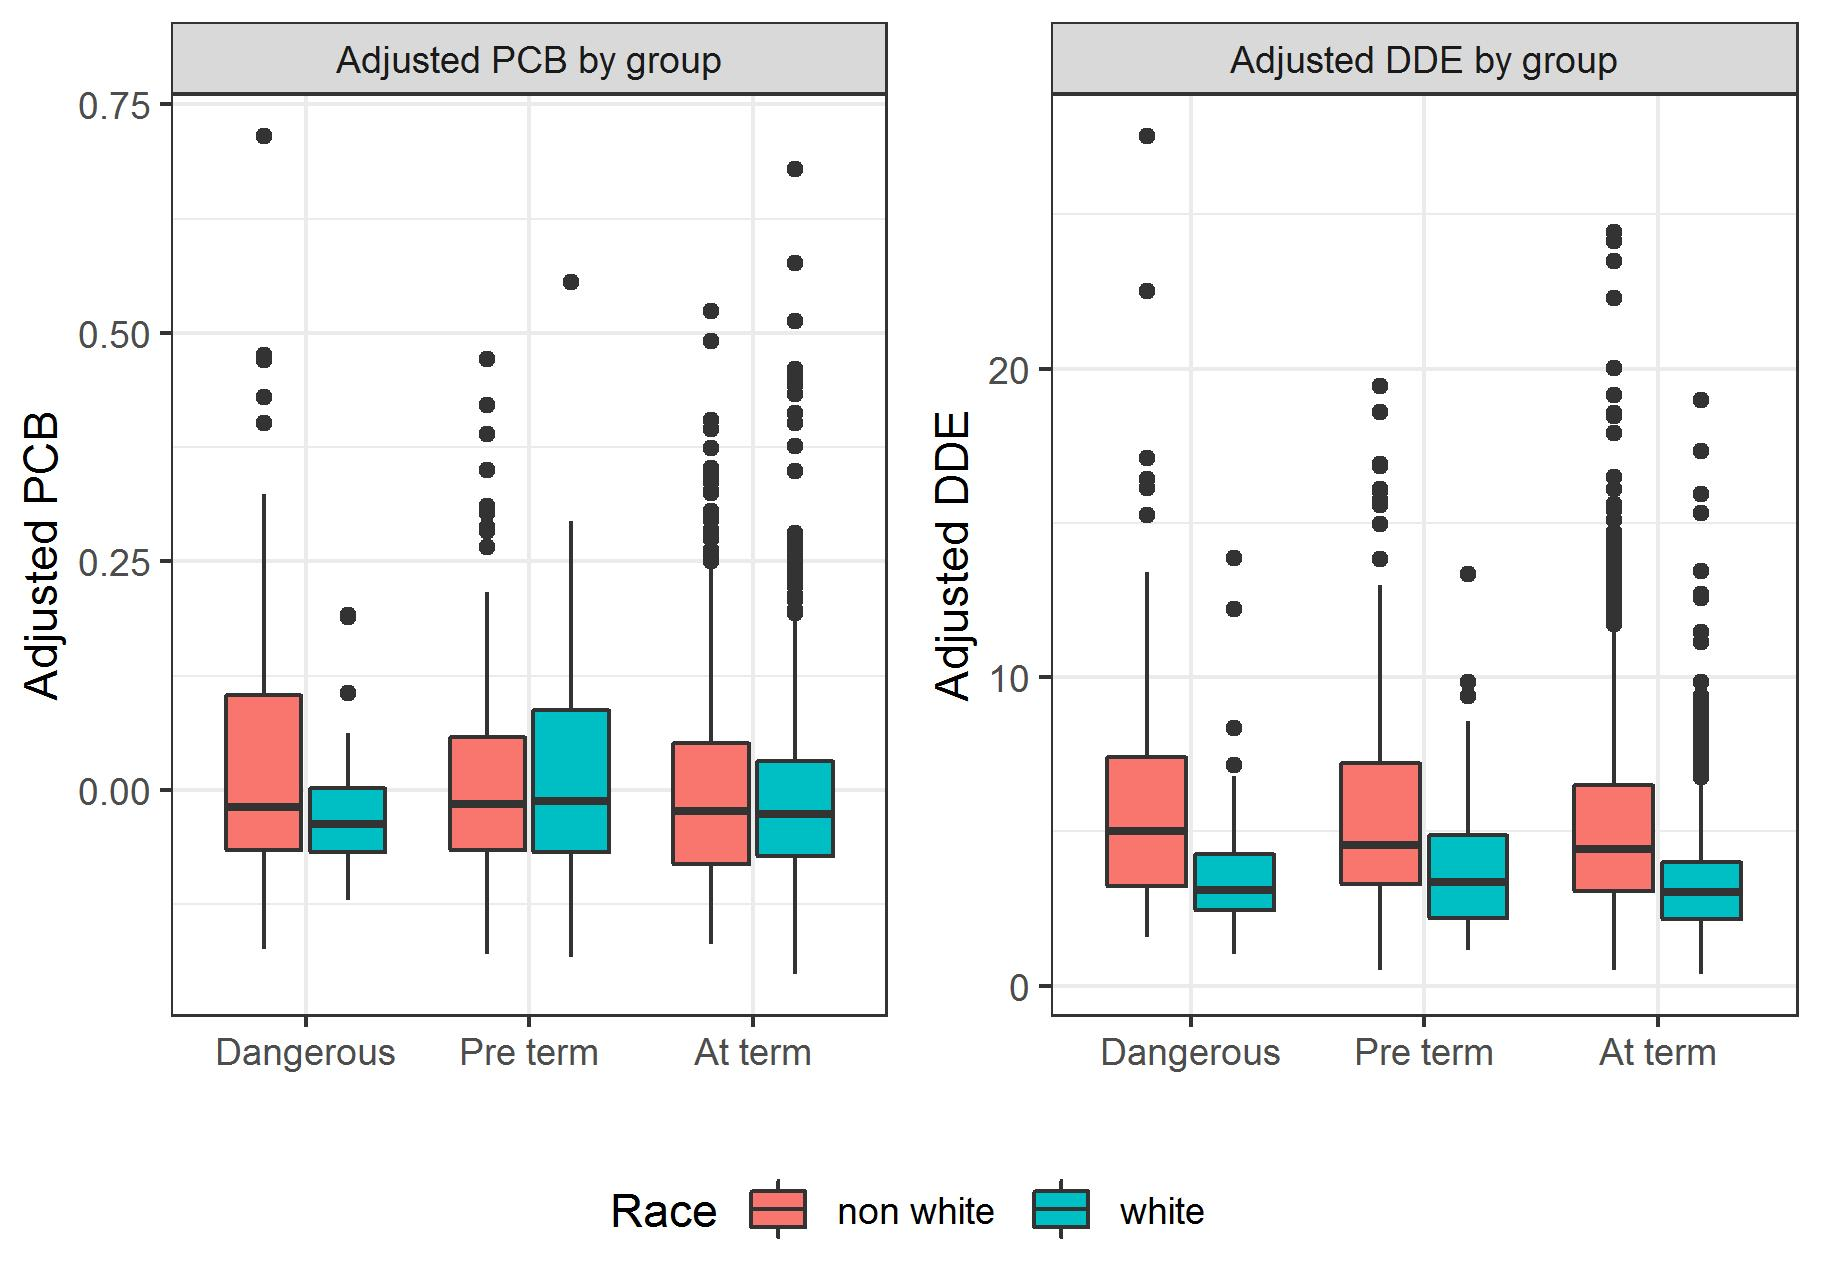
\includegraphics[width=0.5\linewidth]{pcb_corr}
	\label{fig:corr}
\end{figure}

\begin{figure}[htbp]
	\centering
	\caption{Gestational outcome per hospital center.}
	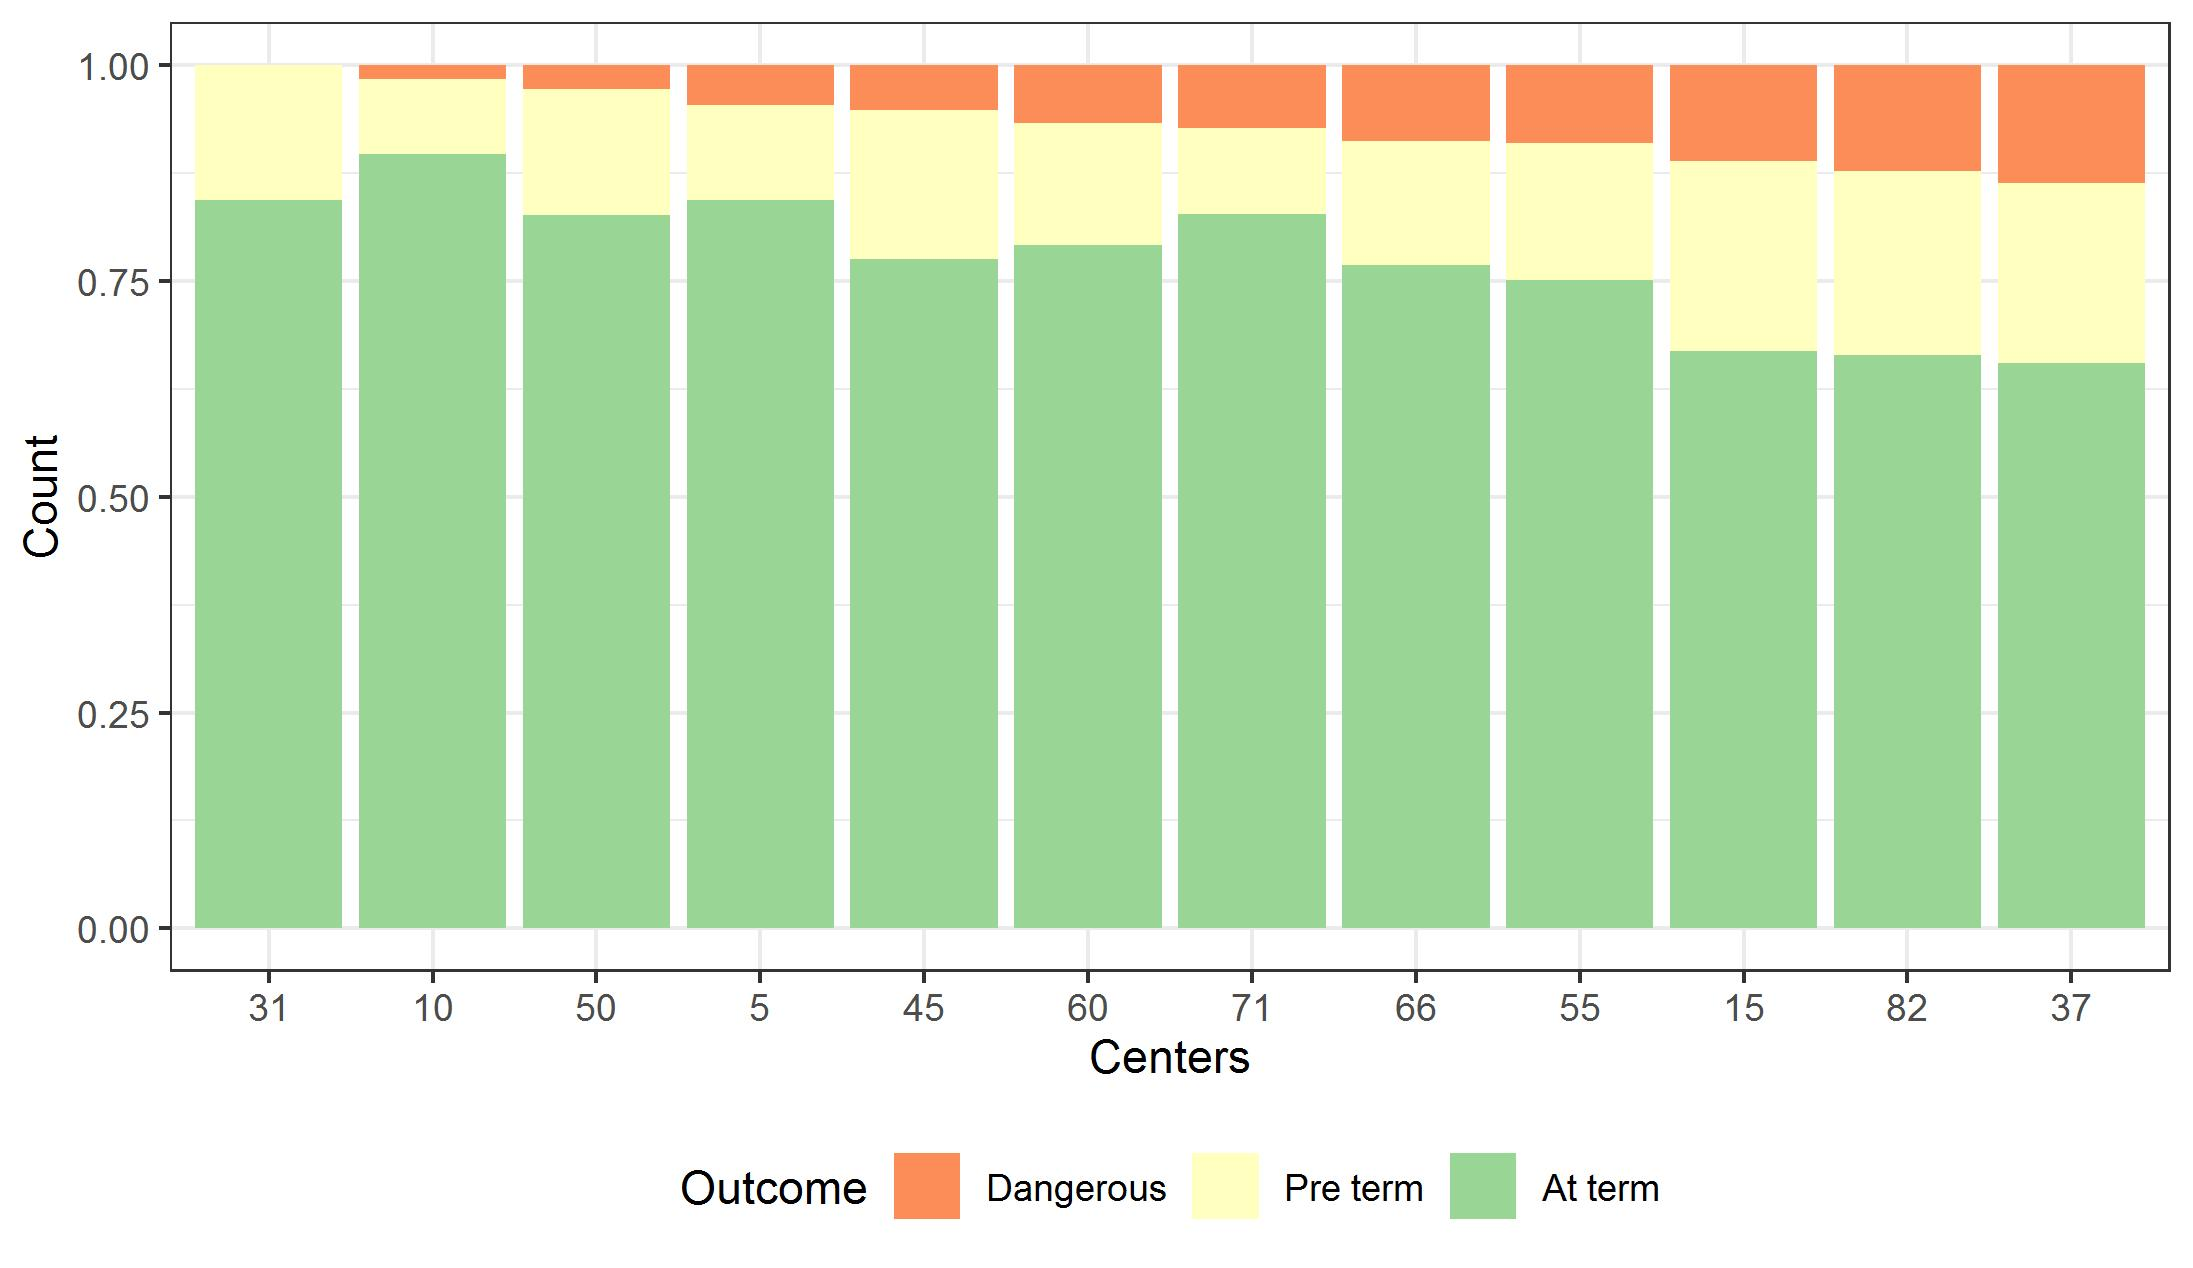
\includegraphics[width=0.7\linewidth]{outcome_per_center}
	\label{fig:center}
\end{figure}

\begin{figure}[htbp]
	\centering
	\caption{Distribution of estimated exposure to PCB and DDE per gestational outcome and per race.}
	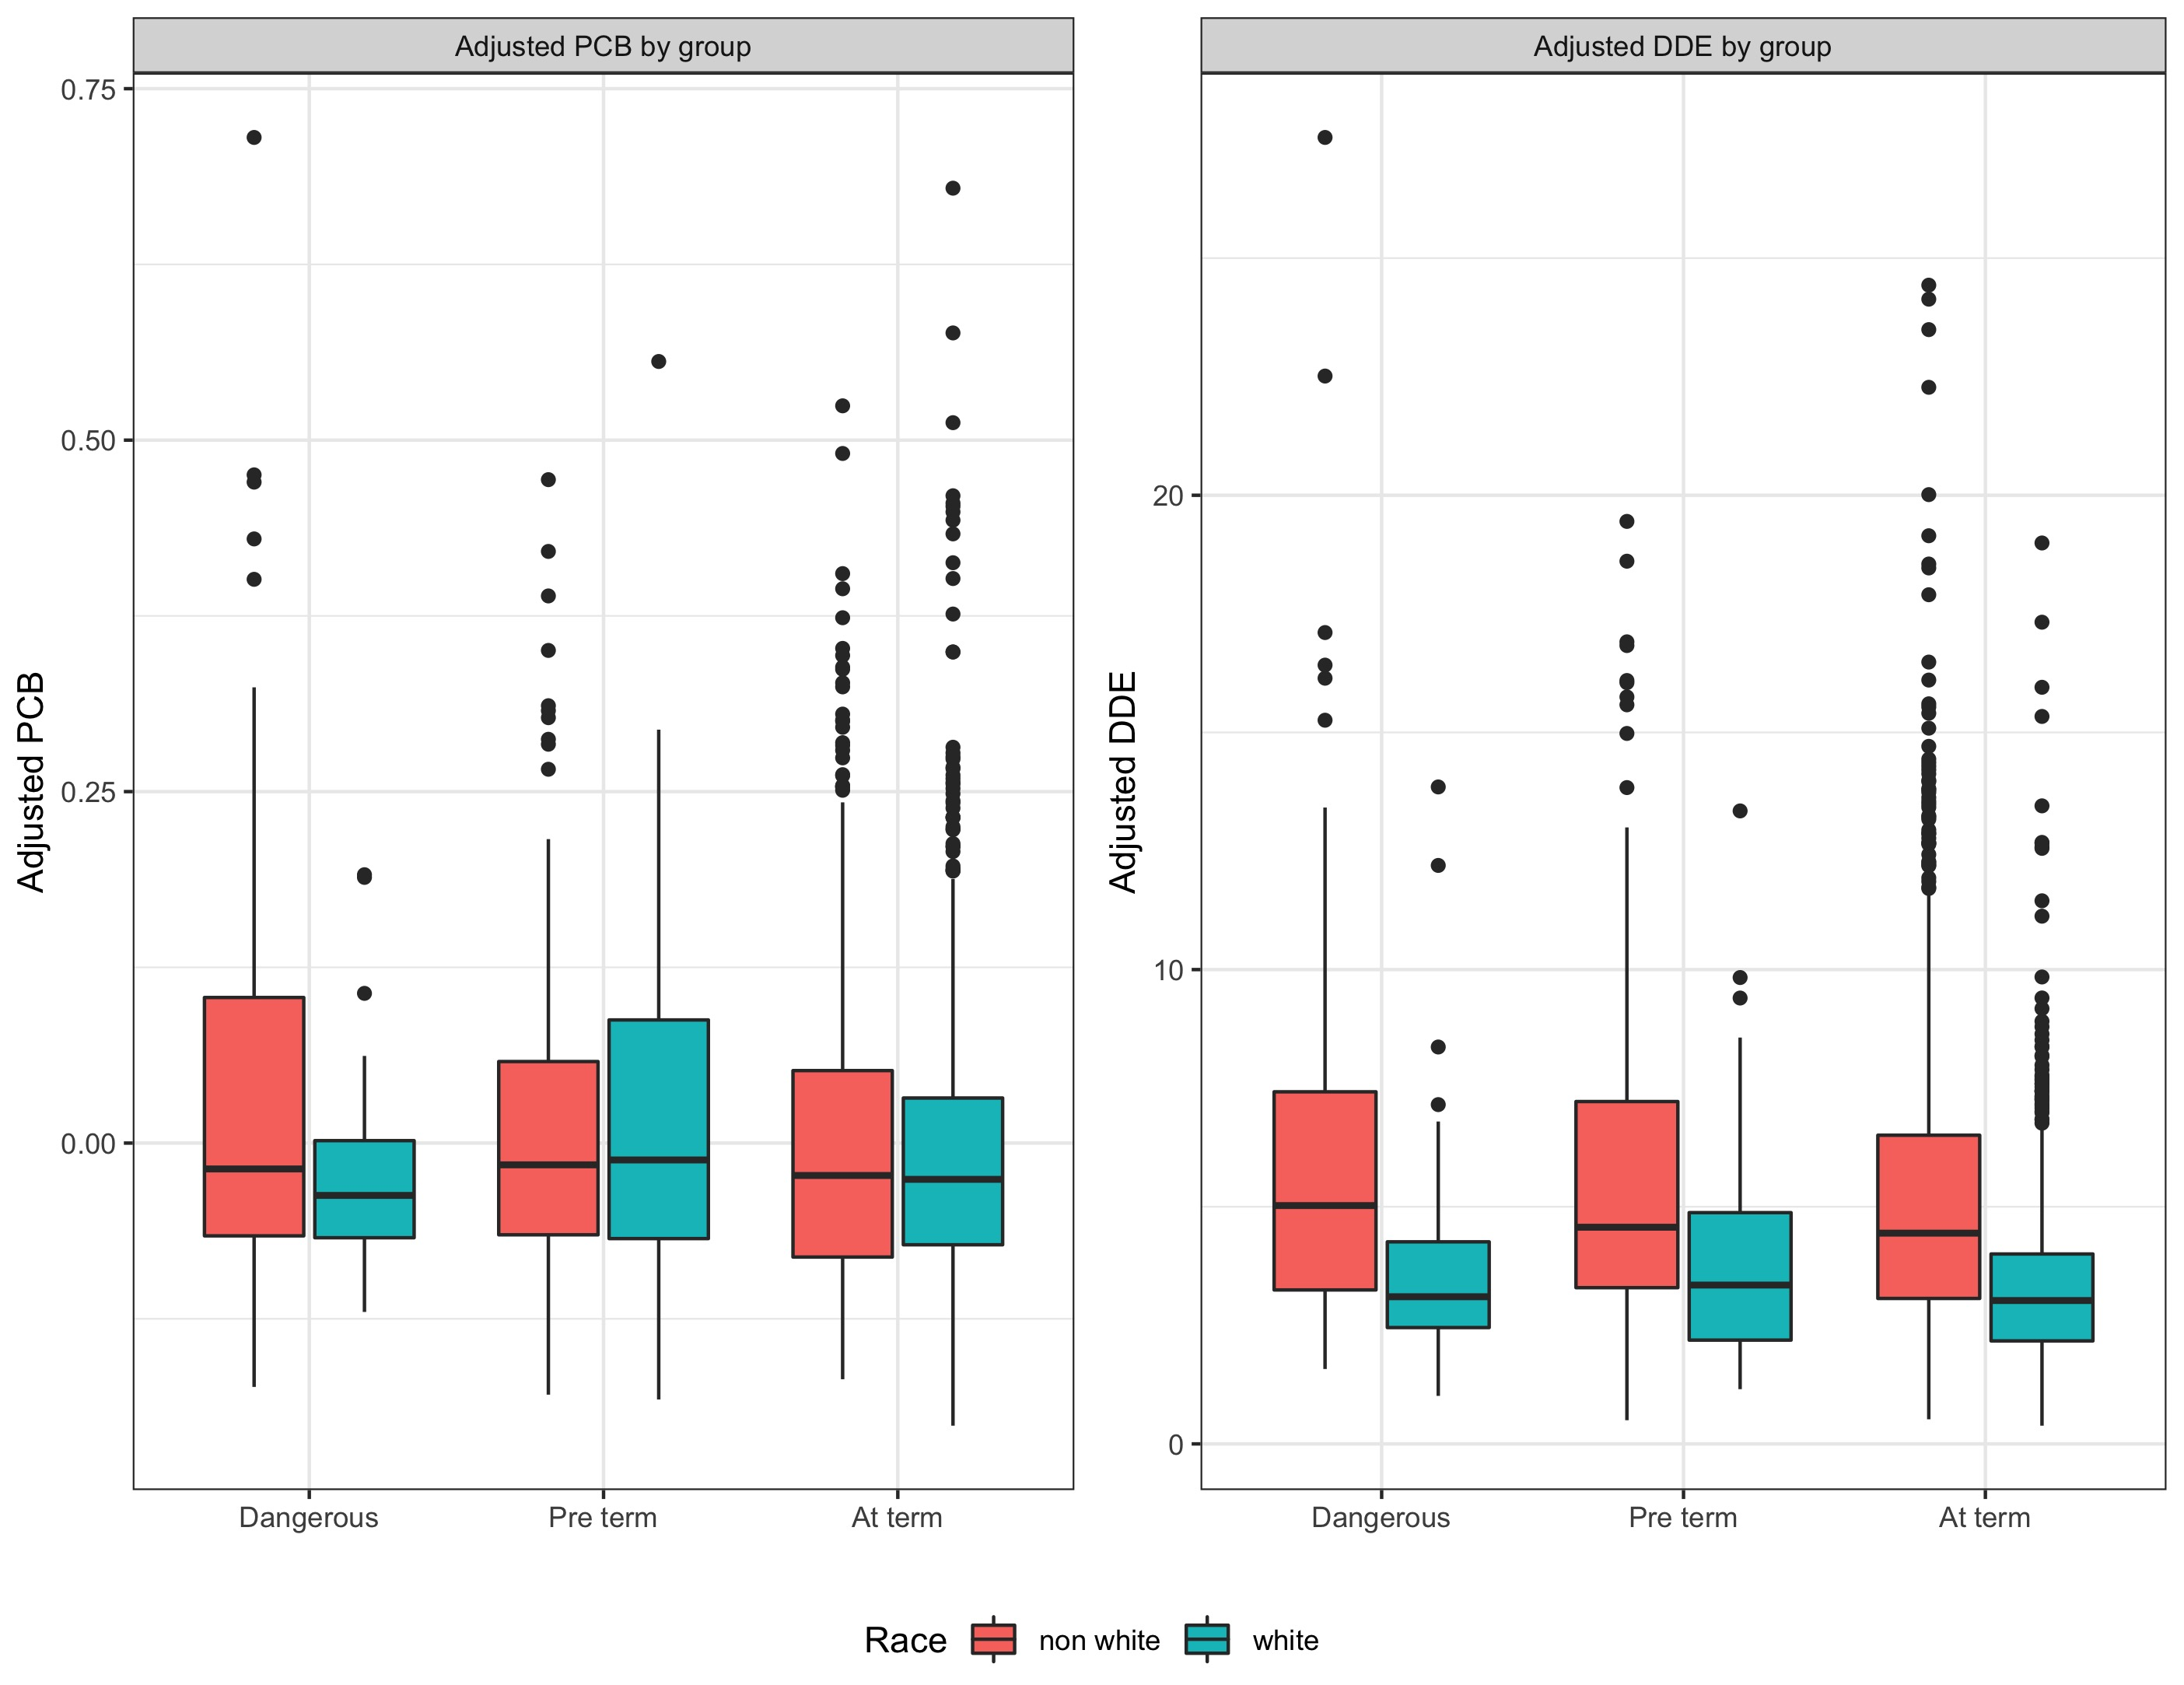
\includegraphics[width=0.7\linewidth]{pcb_dde_per_gest}
	\label{fig:pcb}
\end{figure}

\begin{figure}[htbp]
	\centering
	\caption{Estimated probability of gestation outcomes in function of race, and exposure to DDE and PCB.}
	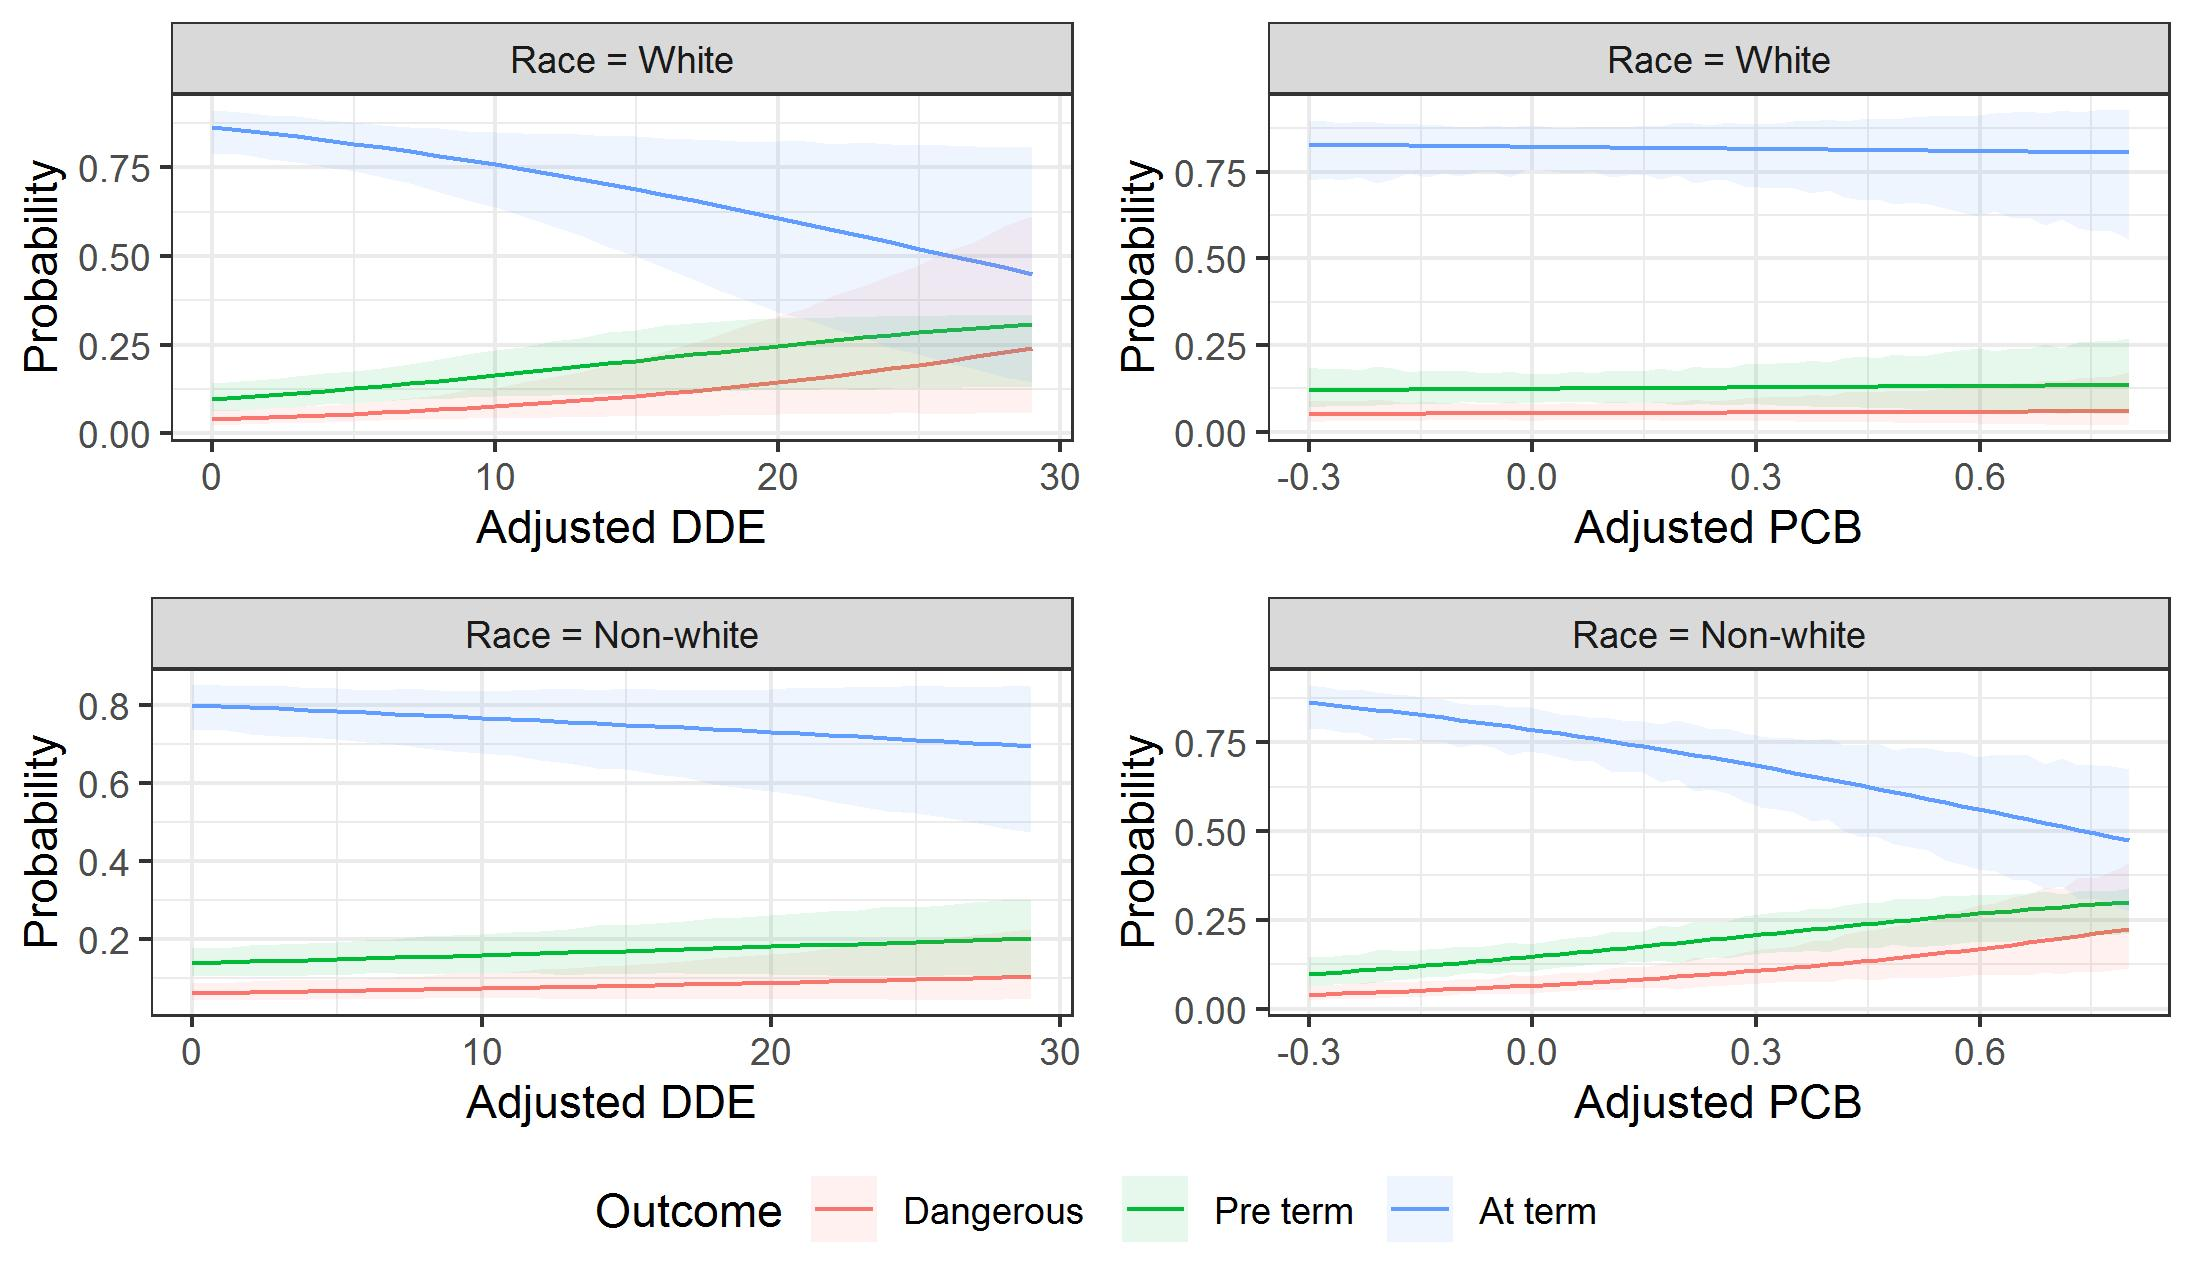
\includegraphics[width=0.7\linewidth]{results}
	\label{fig:results}
\end{figure}



\begin{table}
	\centering
	\label{tab:confints_unif}
	\begin{tabular}{lrrr}
		\toprule
		& mean & 95\% & 5\%\\
		\midrule
		$\text{DDE}_{\text{exposure}}$ & -0.02 & 0.01 & -0.05\\
		$\text{PCB}_{\text{exposure}}$ & -1.76 & -0.72 & -2.75\\
		$\text{DDE}_{\text{exposure}}$*white & -0.05 & 0.02 & -0.12\\
		$\text{PCB}_{\text{exposure}}$*white & 1.60 & 3.26 & -0.02\\
		\bottomrule
	\end{tabular}
	\caption{ 90\% credible intervals and posterior mean of coefficients under a uniform prior.}
\end{table}




\begin{table}[htbp]
	\centering
	\label{tab:confintsR}
	{%
		\subtable[Location $0.3$]{%
			\label{tab:Rfirst}%
			\begin{tabular}{lrrr}
				\toprule
				& mean & 95\% & 5\%\\
				\midrule
				$\text{DDE}_{\text{exposure}}$ & -0.02 & 0.01 & -0.05\\
				$\text{PCB}_{\text{exposure}}$ & -1.87 & -0.81 & -2.87\\
				$\text{DDE}_{\text{exposure}}$*white & -0.06 & 0.02 & -0.12\\
				$\text{PCB}_{\text{exposure}}$*white & 1.69 & 3.36 & 0.08\\
				\bottomrule
			\end{tabular}
		}\qquad
		\subtable[Location 0.5]{%
			\label{tab:Rsecond}%
			\begin{tabular}{lrrr}
				\toprule
				& mean & 95\% & 5\%\\
				\midrule
				$\text{DDE}_{\text{exposure}}$ & -0.02 & 0.01 & -0.05\\
				$\text{DDE}_{\text{exposure}}$ & -1.88 & -0.82 & -2.90\\
				$\text{DDE}_{\text{exposure}}$*white & -0.06 & 0.02 & -0.13\\
				$\text{DDE}_{\text{exposure}}$*white & 1.74 & 3.47 & 0.02\\
				\bottomrule
			\end{tabular}
		}\qquad
		\subtable[Location 0.8]{%
			\label{tab:Rthird}%
			\begin{tabular}{lrrr}
				\toprule
				& mean & 95\% & 5\%\\
				\midrule
				$\text{DDE}_{\text{exposure}}$ & -0.02 & 0.01 & -0.05\\
				$\text{DDE}_{\text{exposure}}$ & -1.94 & -0.88 & -2.96\\
				$\text{DDE}_{\text{exposure}}$*white & -0.06 & 0.01 & -0.13\\
				$\text{DDE}_{\text{exposure}}$*white & 1.77 & 3.60 & 0.04\\
				\bottomrule
			\end{tabular}
		}
	}
{\caption{90\% credible intervals and posterior mean of coefficients under three $R^2$ priors with different locations.}}
\end{table}


\newpage  % ensures that all figures remain together in appendix B

%%%%%%%%%%%%%%%%%%%%%%%%%%%%%%%%% BOX COX
\section{Box-Cox analysis for lipid adjustment.}

Part of the issue with the exposures of interest in our study (DDE and PCB) is that the substances are lipophilic. This may require to adjust their measurement by the total serum lipid concentration in the blood, so to have an estimate for the excess exposure that comes from the environment. The work by \cite{Li_Long_Duns} suggests a possible correction based on a Box- Cox analysis. In particular, let $s_i$ be the measure for the total lipids serum concentration, and $x_i$ the exposure. The adjusted exposure can be computed by setting 
\begin{equation}
x_i^* = x_i/g(s_i)
\end{equation} 
where $g$ is a function to be estimated. A way to do this is by letting $g$ being equal to the Box-Cox correction, that is
\begin{equation}
g(s_i,\lambda) = 
\begin{cases} 
\frac{s_i^\lambda-1}{\lambda} & \lambda \neq 0 \\
\log(s_i) & \lambda =0 
\end{cases}
\end{equation}
Assuming that there is a unique $\lambda$ correction for each level of chemical exposure, we can plot the Log-Likelihood across varying levels of $\lambda$, and then choose the one that maximizes it. In such a way, we can get rid of the potential case in which serum lipids do not have any impact on the covariate. Under such a scenario, the likelihood should pick at a $\lambda$ that minimizes the effect of lipids (making the effect of $x_i$ and $x_i^*$) practically identical. 

Following the above reasoning, we plot the Log-Likelihood across varying levels of $\lambda$  under the transformations
\begin{equation}
\textrm{DDE}_{\text{exposure}} = \frac{DDE}{g(\text{lipid})} \qquad \textrm{PCB}_{\text{exposure}} = \frac{PCB}{g(\text{lipid})}
\end{equation}


\begin{figure}[htbp]
	\centering
	\caption{Log-likelihood for different values of $\lambda$.}
	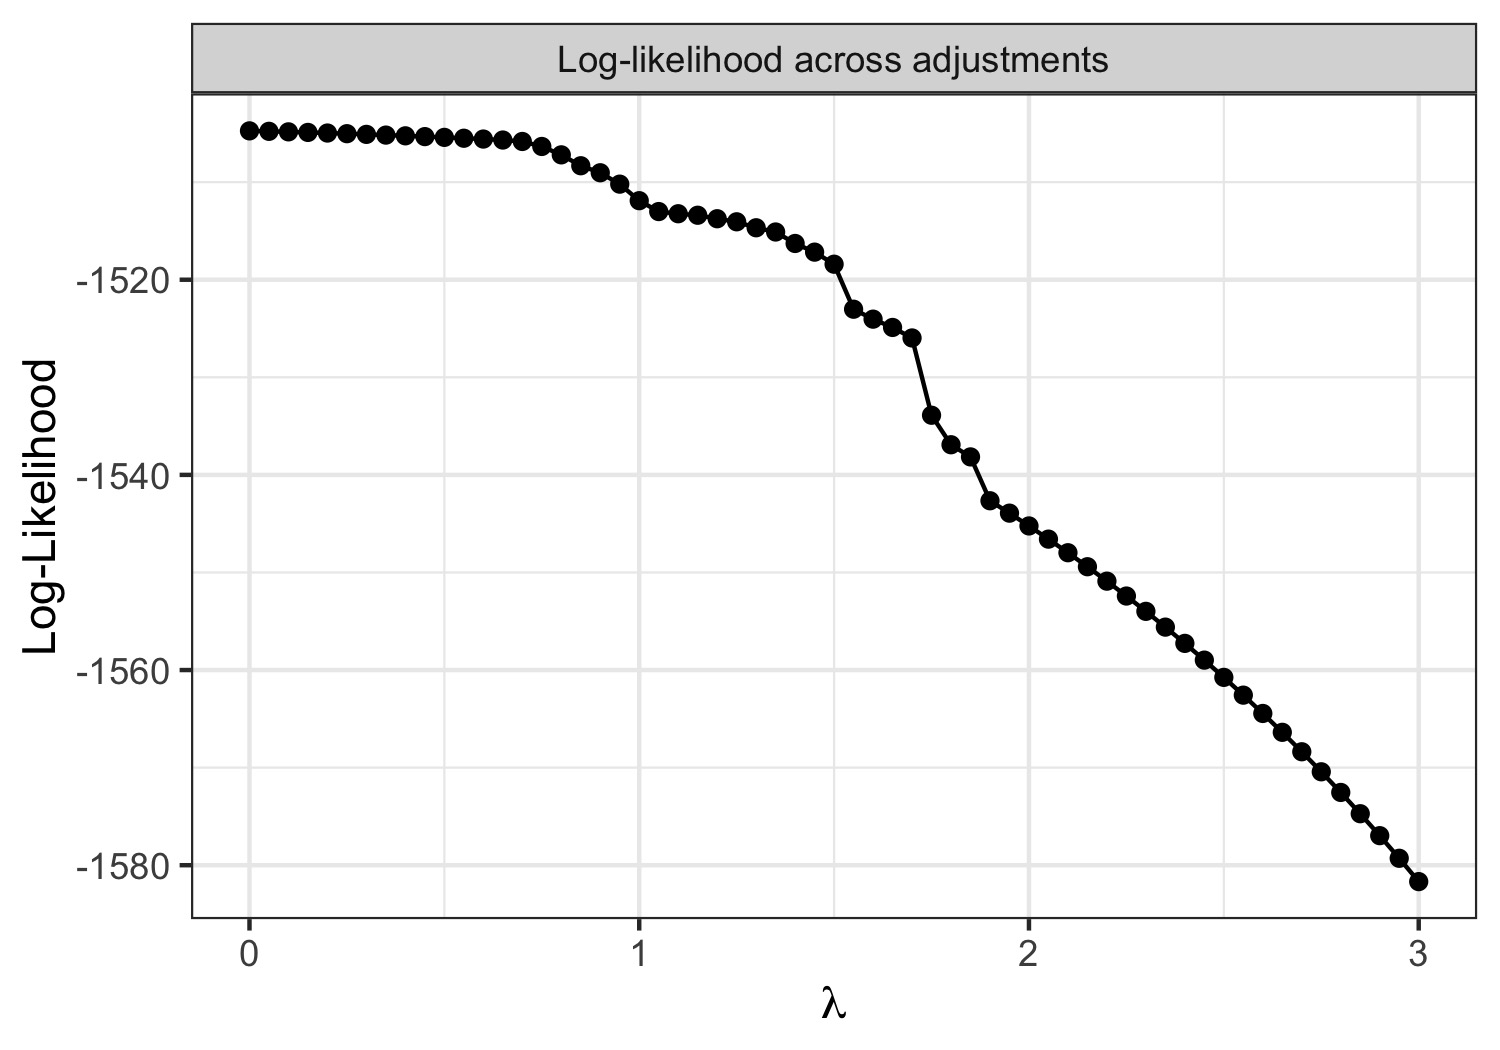
\includegraphics[width=0.7\linewidth]{BocCox}
	\label{fig:boxcox}
\end{figure}

We can see that the value at which the log likelihood peaks is 0. This suggests that a $\log$-transformation o  both variables in preferable. Note that we do not consider any negative transformation for interpretability reasons. 

%%%%%%%%%%%%%%%%%%%%%%%%%%%%%%%%% MODEL CHECKING
\section{Model Checking}

Since the ordinal data is used, the common residual model checking plot is no longer applicable. Instead, the surrogate residual method suggested by \cite{Liu2018} is used. 

Latent variables $Z$ can be used to parameterize the Bayesian logistics model. Specifically, $Z=-X\beta+\epsilon$ and $Y=j$ if $Z\in[\alpha_{j-1},\alpha_{j}]$, where $\epsilon$ is a random variable with cumulative distribution $G(\cdot)$ and $\alpha_{j}$ is some threshold value. $G^{-1}(\cdot)$ is the link function of the model. Surrogate residual is defined as $R_S=S-E(S|X)$, where $S$ is some continuous variable generated from the conditional distribution of latent variables $Z$ given observation $Y$. If the model assumptions are satisfied, the surrogate residual $R_S$ should display three characteristics: 

\begin{enumerate}
	\item $E(R_S|X)=0$
	\item $Var(R_S|X)=c$, the conditional variance of $R_S$ is constant.
	\item The empirical distribution of $R_S$ resembles an explicit distribution that is related to the link function $G^{-1}(\cdot)$. Specifically, $R_S\sim G(c+\int ud G(u))$ and $R_S$ is independent of $X$, where $c$ is a constant.
\end{enumerate}

To explain more straightforwardly, if the model assumptions are satisfied, $R_S$ should distribute evenly around 0, independent of $X$. Besides, the empirical quantiles of $R_S$  should match those of the theoretical distribution.

The scatterplot (Figure\ref{fig:surrogateresid}) indicates that feature 1 and 2 are roughly satisfied. The QQ plot indicates that feature 3 is roughly satisfied, although the tail of our sample distribution is lighter than that of the theoretical one. 


\begin{figure}
	\centering
	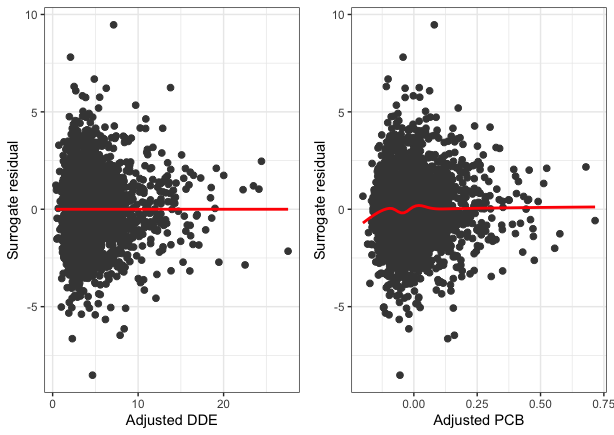
\includegraphics[width=0.7\textwidth]{Surrogate_residuals.png}
	\caption{Surrogate residuals of DDE and PCB}
	\label{fig:surrogateresid}
\end{figure}

\begin{figure}
	\centering
	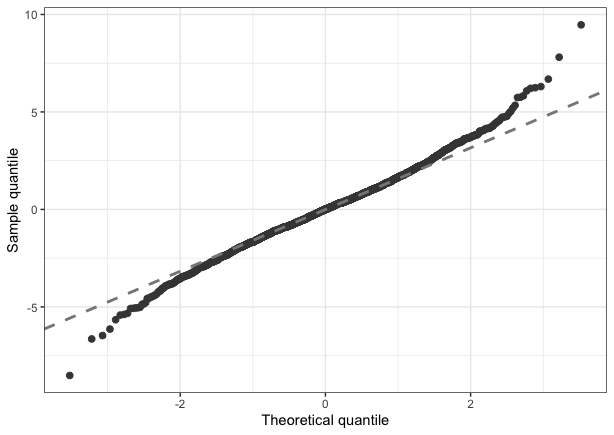
\includegraphics[width=0.7\textwidth]{qqplot.png}
	\caption{QQ plot of the Surrogate residuals}
	\label{fig:qqplot}
\end{figure}

\section{Full Model Output}
The comprehensive output of our model is also included (See Table \ref{tab:fullcoef} for credible intervals and Figure \ref{fig:hists} for the histogram). Although the effects of variables other than $\text{DDE}_{\text{exposure}}$ and $\text{PCB}_{\text{exposure}}$ an are not the focus on this report, we can still interpret the coefficients of variables like intercepts and center. 
\begin{itemize}
	\item Intercept: when a subject is non-white, measured at center 5, doesn't smoke, and exposed to 0 level of DDE and PCB, her 90\% credible interval for the risk of dangerous preterm is $\frac{1}{1+e^{[-3.24, -2.54]}}*100\%=[3.77\%, 7.31\%]$.  90\% credible interval for the dangerous preterm or preterm is $\frac{1}{1+e^{[-1.88, -1.22]}}*100\%=[13.24\%, 22.79\%]$.
	
	\item Center: There are clear heterogeneity across centers. Center$5$ is chosen to be the baseline here. Center 15, 37, 82 are significantly different from the baseline because their 90\% credible intervals do not cover 0.
\end{itemize}

\begin{table}
	\centering
	\begin{tabular}{lrrr}
		\toprule
		 & 5\% & 95\% & mean\\
		\midrule
		$\text{DDE}_{\text{exposure}}$ & -0.05 & 0.01 & -0.02\\
		$\text{PCB}_{\text{exposure}}$ & -2.73 & -0.75 & -1.76\\
		race\_aggwhite & 0.10 & 0.85 & 0.47\\
		center10 & -0.13 & 0.77 & 0.31\\
		center15 & -1.11 & -0.28 & -0.69\\
		\addlinespace
		center31 & -0.25 & 0.80 & 0.26\\
		center37 & -1.01 & -0.32 & -0.65\\
		center45 & -0.42 & 0.35 & -0.04\\
		center50 & -0.54 & 0.23 & -0.16\\
		center55 & -0.78 & 0.08 & -0.35\\
		\addlinespace
		center60 & -0.66 & 0.16 & -0.25\\
		center66 & -0.48 & 0.19 & -0.14\\
		center71 & -0.46 & 0.28 & -0.09\\
		center82 & -1.09 & -0.29 & -0.69\\
		smoking\_status1 & -0.31 & 0.00 & -0.16\\
		\addlinespace
		$\text{DDE}_{\text{exposure}}$*white & -0.12 & 0.02 & -0.05\\
		$\text{DDE}_{\text{exposure}}$*white & 0.01 & 3.21 & 1.61\\
		\bottomrule
		\end{tabular}
	\label{tab:fullcoef}
	\caption{90\% credible intervals for all coefficients, under the uniform prior}
\end{table}

\begin{figure}
	\centering
	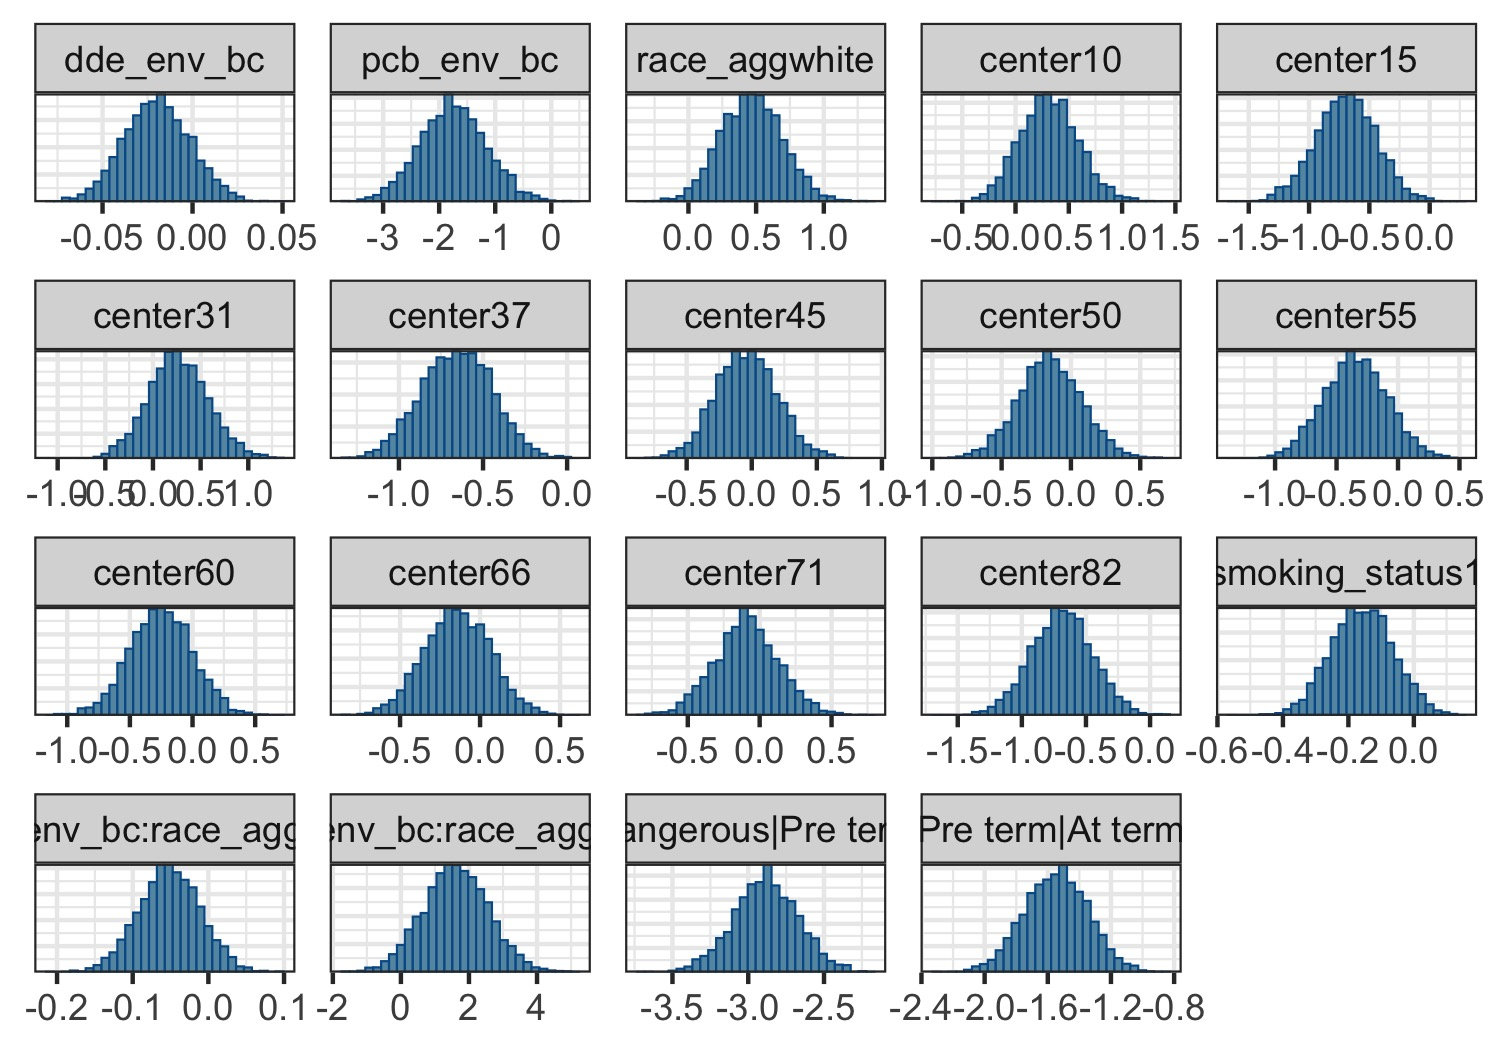
\includegraphics[width=\textwidth]{hists.jpeg}
	\caption{Histogram of posterior draws.}
	\label{fig:hists}
\end{figure}

%\bibliography{bibliography}
\end{document}